%!TEX root = stokes_paper.tex

\section{Examples \label{sec:results}}
In this section, we test the lightning Stokes solver on various problems found in the literature. For each example, we present contour plots of the stream function $\psi$ superimposed on a color plot of the velocity magnitude $\sqrt{u^2+v^2}$. We use black contours for the main flow, which we also regard as the first Moffat eddy, and yellow contours for the subsequent eddies. We mark the poles near the corners by red dots. The plots of the linear least-squares (weighted) residual on the boundary indicate root-exponential convergence as expected. We also provide a close-up of each eddy with contours at 0, 0.05, 0.35, 0.65, and 0.95 relative to the maximum absolute value of $\psi$, and a log-log plot of $\abs{\psi}$ along the corner bisector to identify how many eddies are resolved by our numerical method.

Reversing the sign of the boundary data $(h,k)=(\psi_0(z_i), U_t(z_i))$ and $\vec{g}=(U(z_i), -V(z_i))$ would have the effect of reversing the direction of the flow, since \eqref{eq:bih}--\eqref{eq:bcs} is linear. Therefore, the streamline pattern and the velocity magnitude plot would appear unaltered.


\begin{example}[Lid-driven square cavity.]
\label{ex:square}
As our first example, in Figure \ref{fig:ldc} we present a square lid-driven cavity, where the fluid is enclosed between fixed walls except that one of them moves tangentially to the fluid as the forcing mechanism. Here, the domain is the square $\Omega=[-1,1]^2$, where we have a no-slip BC with $\psi=0$ on the bottom, left and right edges, and we impose $u=1$ and $\psi=0$ on the top edge. Since the gradient data $k(x,y)$ is discontinuous, $\psi$ presents point singularities at $(\pm 1, 1)$. On the bottom corners, $(\pm 1,-1)$, there are (weaker) point singularities caused by the formation of Moffatt eddies, and our adaptive strategy put fewer poles at these corners.

Figure \ref{fig:ldc_loglog} shows a log-log plot of $\abs{\psi}$ along the $45^\circ$ line. The asymptotic curve was obtained by fixing the smallest non-trivial root inside the first quadrant of \eqref{eq:roots} for $2\alpha=90^\circ$, namely $\lambda=3.74 + 1.12i$, and fitting via least-squares the amplitude and phase factor $C = A_0 r_0^{-\lambda}$ from the second eddy to the origin.  The exact solution would follow the asymptotic trend all the way to $r=0$, our numerical method achieves this roughly up to the level of accuracy obtained in the boundary fitting least-squares problem, which explains why the zero contour for the third eddy is not present in Figure \ref{fig:ldc}. 
\begin{figure}[H]
\centering
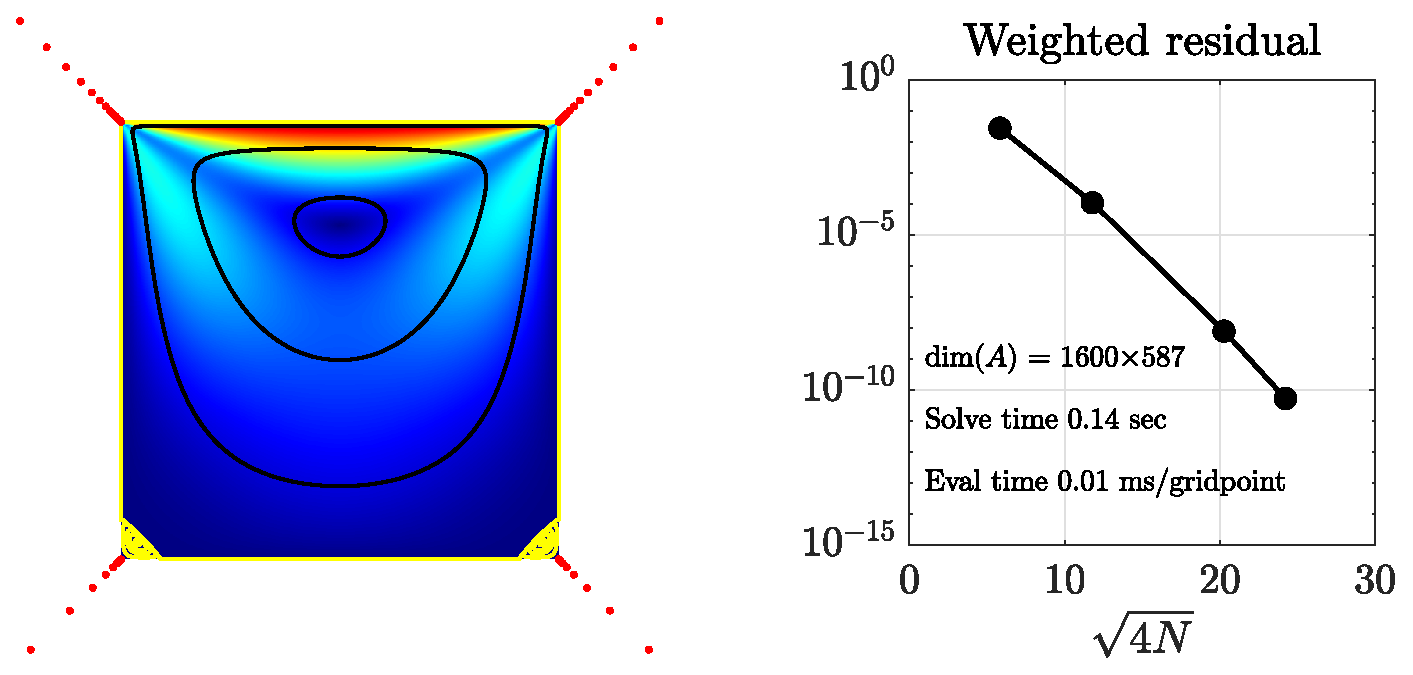
\includegraphics[width=\linewidth]{Figures/ldc}

\vspace{2em}
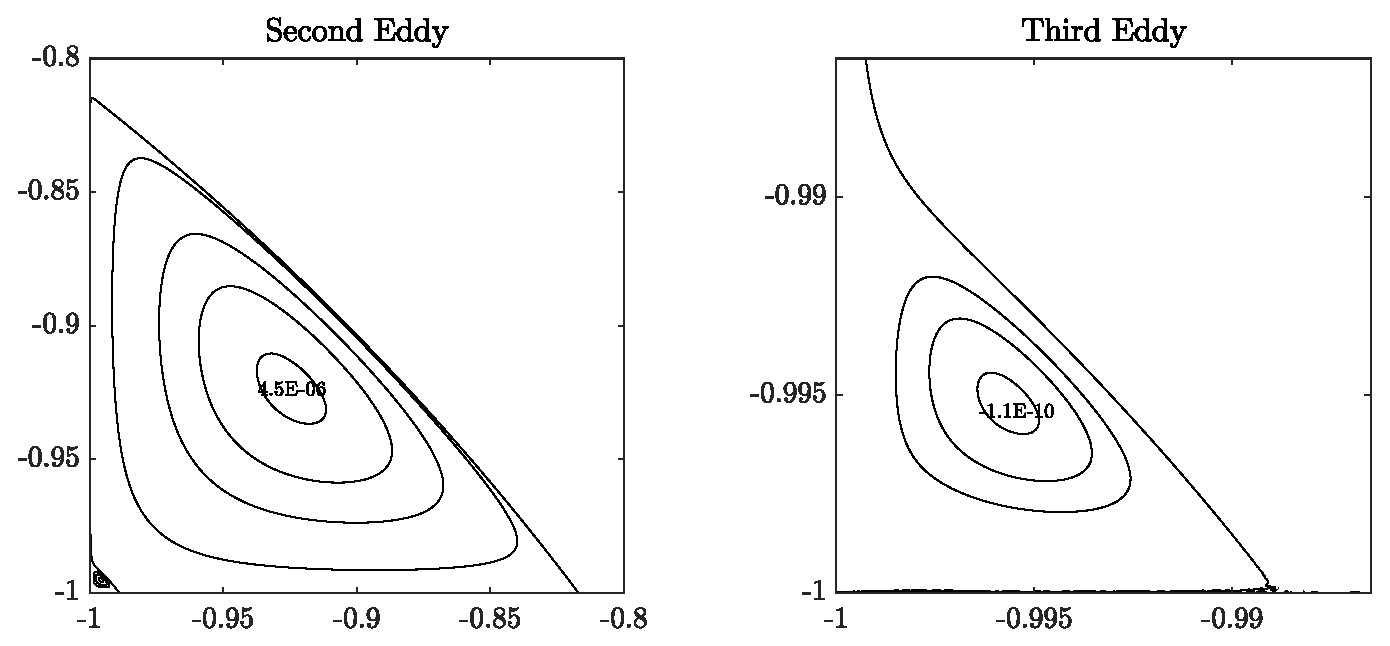
\includegraphics[width=\linewidth]{Figures/ldc_eddy}

\caption{Stokes flow in a square lid-driven cavity solved to 10-digit accuracy in 0.14 secs. on a laptop. Stream contours and velocity magnitude (top left), convergence (top right), and close-ups of the eddies (bottom).}
\label{fig:ldc}
\end{figure} 
\begin{figure}[H]
\centering
\includegraphics[width=0.9\linewidth]{Figures/ldc_loglog}
\caption{Stream function log-log plot along the $45^\circ$ line for Example \ref{ex:square}. The length scale $L=2\sqrt{2}$ corresponds to the diagonal of the cavity. The computed solution matches the asymptotic approximation to plotting accuracy over an amplitude range of ten orders of magnitude.}
\label{fig:ldc_loglog}
\end{figure}

\end{example}


\begin{example}[Lid-driven triangular cavity.]
\label{ex:triangle}
In terms of boundary conditions and singularities, the situation in Figure \ref{fig:wedge} is quite similar to the one depicted in the previous example, except that the bottom wall has now been collapsed into a single point. Here, the domain is the isosceles triangle with unit leg and vertex angle $2\alpha = 28.5^\circ$, which corresponds to $\lambda = 9.49 + 4.43i$. The fact that the corner is sharper than in the previous example introduces a faster decay rate and a higher frequency in the eddies, since both the real and imaginary parts of $\lambda$ have been increased. As a consequence, four eddies can be observed without the need of a close-up.

This particular setup was chosen for direct comparison with experimental images from Taneda \cite[Fig.~19]{taneda79}, also featured in \cite[Fig.~10]{vandyke82}, where he used a very similar setup driven by a rotating cylinder with Reynolds number $1.7\times10^{-1}$. His imagining technique employed glycerin as the working fluid with suspended aluminum particles and a photographic exposure time of 90 minutes. Only the first two eddies were visible from the experiment, as it is extremely difficult to visualize two Moffat eddies. According to Taneda, ``the reason is that the relative intensity of successive vortices is the order $10^3$ and therefore the photographic exposure necessary to visualize two successive vortices is about $10^3$ times that necessary to visualize a single vortex.''

\begin{figure}[H]
	\centering
	\begin{tikzpicture}
	\usetikzlibrary{calc}
	\node(picA){
	\begin{minipage}{0.45\linewidth}
	\centering
	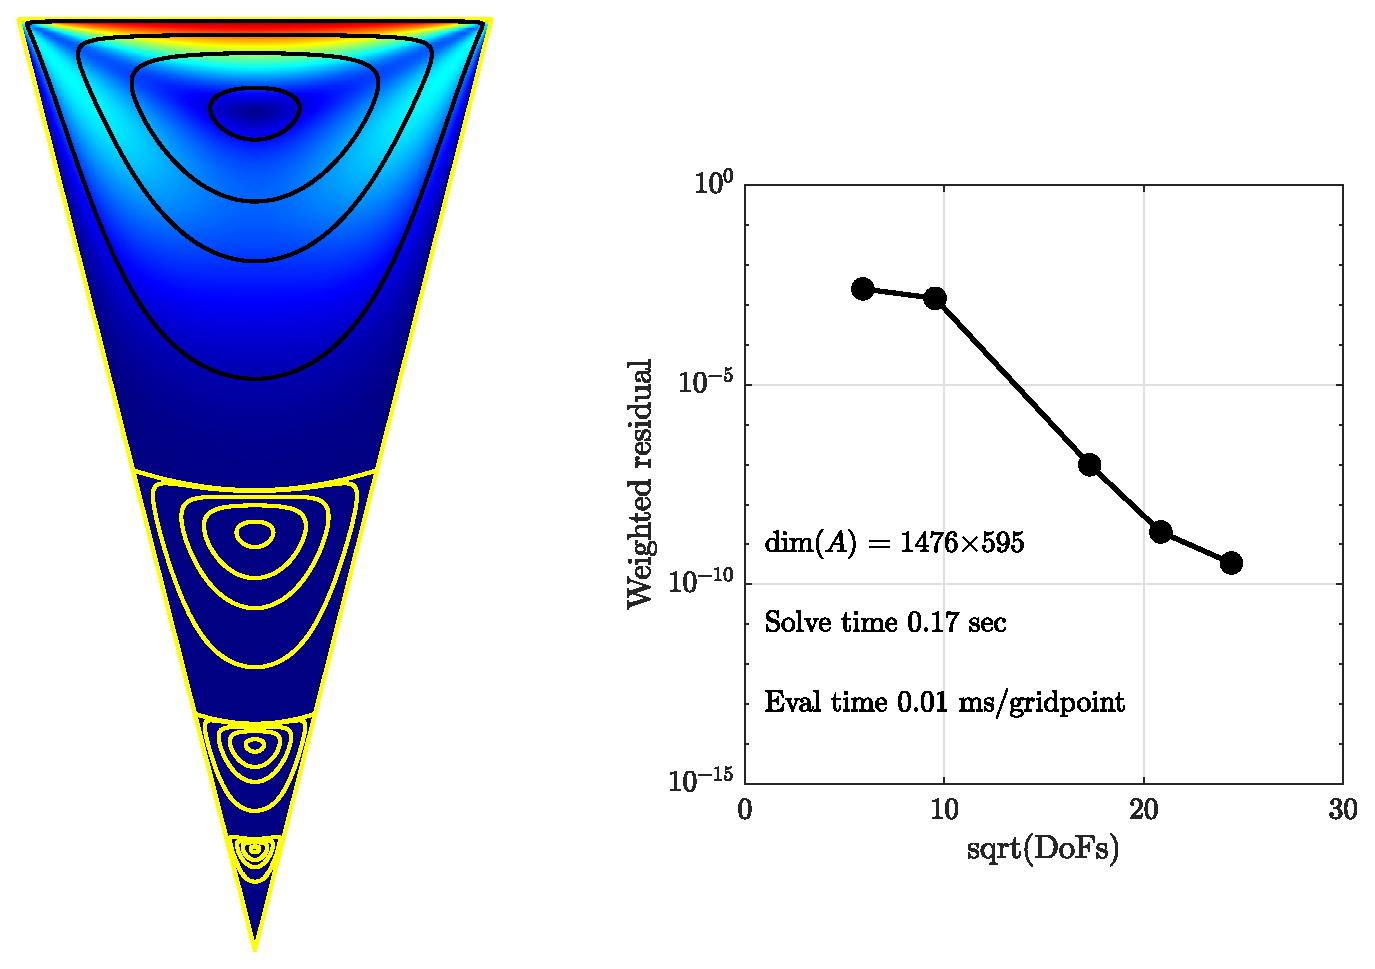
\includegraphics[width=\linewidth]{Figures/wedge}
	\end{minipage}
	\hspace{0.1\linewidth}
	\begin{minipage}{0.45\linewidth}
	\centering
	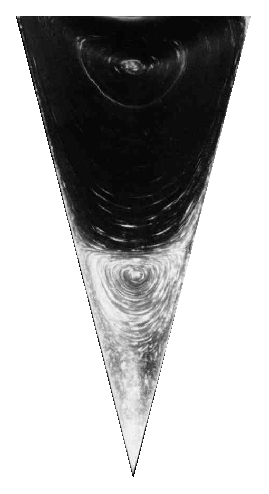
\includegraphics[width=0.6\linewidth]{Figures/wedge_exp}
	\end{minipage}	
	};
	\node at($(picA.south) + (0,3)$){
		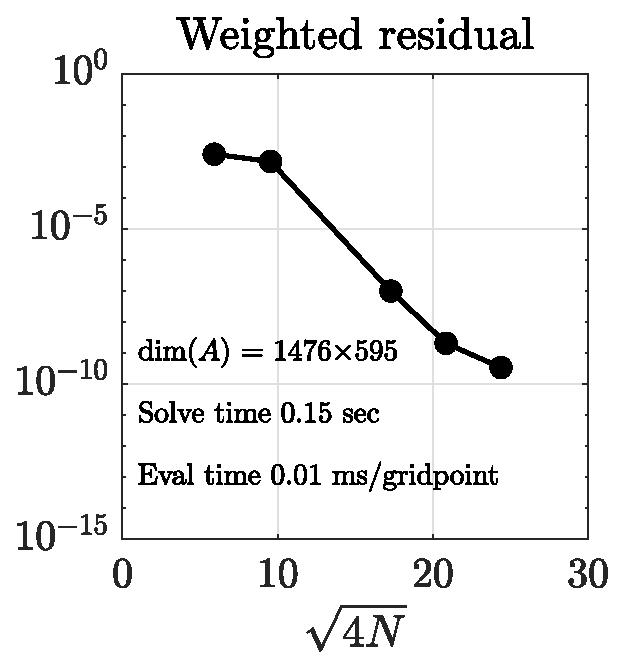
\includegraphics[width=0.4\linewidth]{Figures/wedge_conv}
	};
	\end{tikzpicture}    
	\caption{Stokes flow inside an isosceles triangle of vertex angle $2\alpha=28.5^\circ$.}
	\label{fig:wedge}
\end{figure} 
\begin{figure}[H]
	\centering
	\includegraphics[width=0.9\linewidth]{Figures/wedge_loglog}
	\caption{Stream function log-log plot along the vertical line for Example \ref{ex:triangle}. The length scale $L=\cos{\alpha}$ corresponds to the height of the triangle. The computed solution matches the asymptotic approximation to plotting accuracy over an amplitude range of ten orders of magnitude.}
	\label{fig:wedge_loglog}
\end{figure}
\end{example}


\begin{example}[Flow over a step.]
\label{ex:step}
In Figure \ref{fig:step} we have the L-shaped domain $\Omega = [-1,0] \times [0,1] \cup [0,5]\times[-1,1]$ that resembles a finite section of a pipe with a sudden expansion or a step. Fully-developed parabolic profiles are imposed at the inflow and outflow such that mass flow is conserved, i.e. $(u,v)=(1-(2y-1)^2,0)$ at $x=-1$, $(u,v)=((1-y^2)/2,0)$ at $x=5$, and for the remaining surfaces we impose a no-slip BC with $\psi_0=2/3$ at $y=1$ and $\psi_0=0$ on the other walls. We observe more poles clustered near the re-entrant corner $(0,0)$, where the pressure becomes unbounded. 

This time the main flow is not an eddy, since we have imposed inflow and outflow BCs. The corner at $(0,-1)$, on which the Moffatt eddies appear, forms a $90^\circ$ angle as in Example \ref{ex:square}. And once again we are able to resolve two additional eddies, only that this time the zero contour on the second eddy can be plotted.

In order to make this example run with lightning speed, it was crucial to introduce a fake vertex at $(0,1)$. Otherwise, as in the Laplace problem, we observed that the use of Arnoldi plays a crucial role for convergence.
\begin{figure}[H]
	\centering
	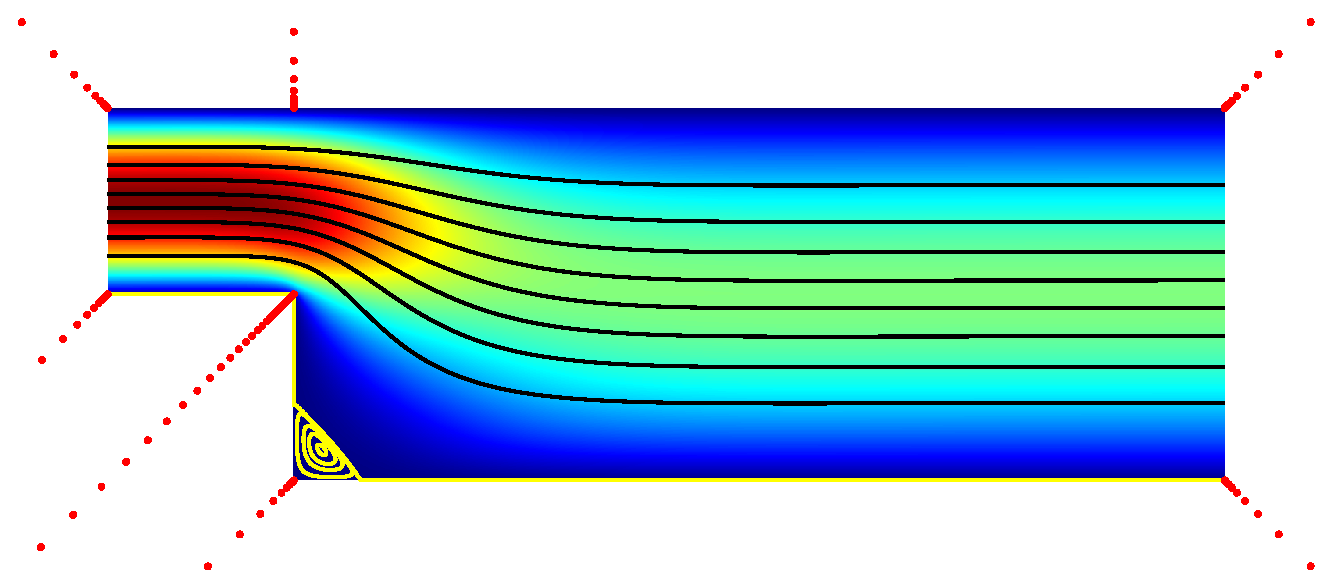
\includegraphics[width=\linewidth]{Figures/step}
	
	\vspace{2em}
	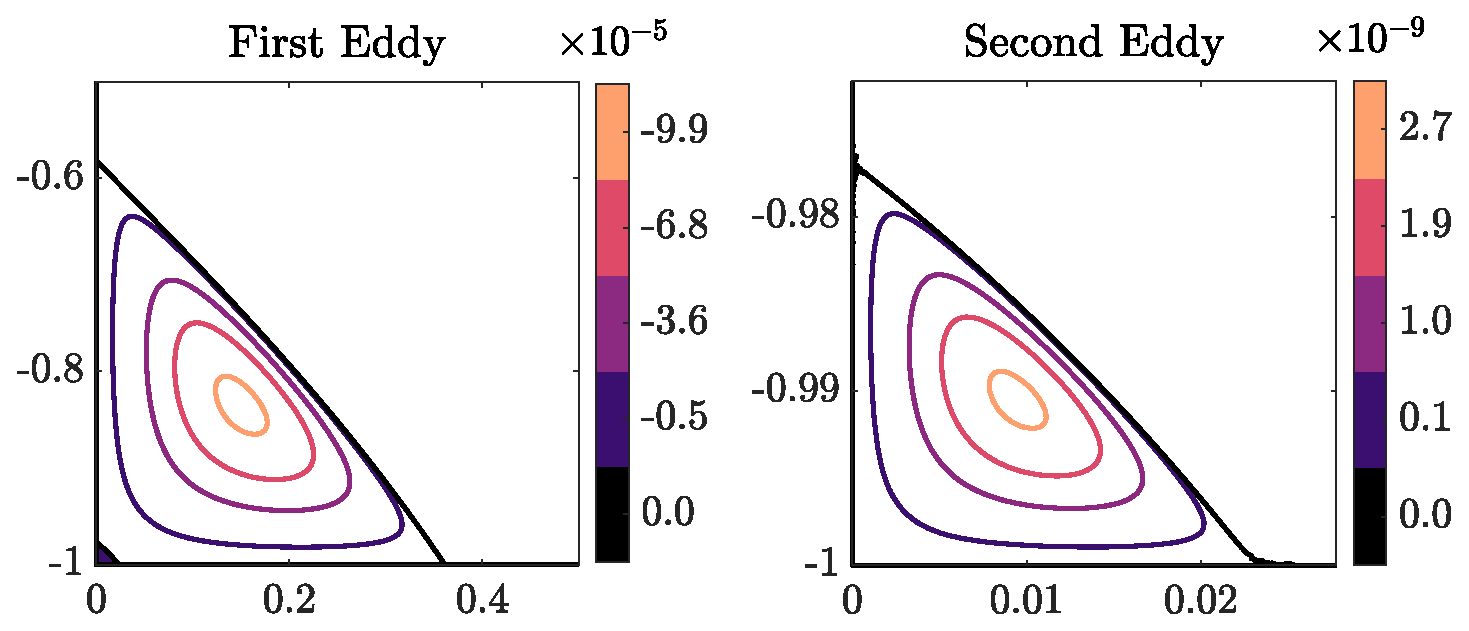
\includegraphics[width=\linewidth]{Figures/step_eddy}
	
	\vspace{2em}
	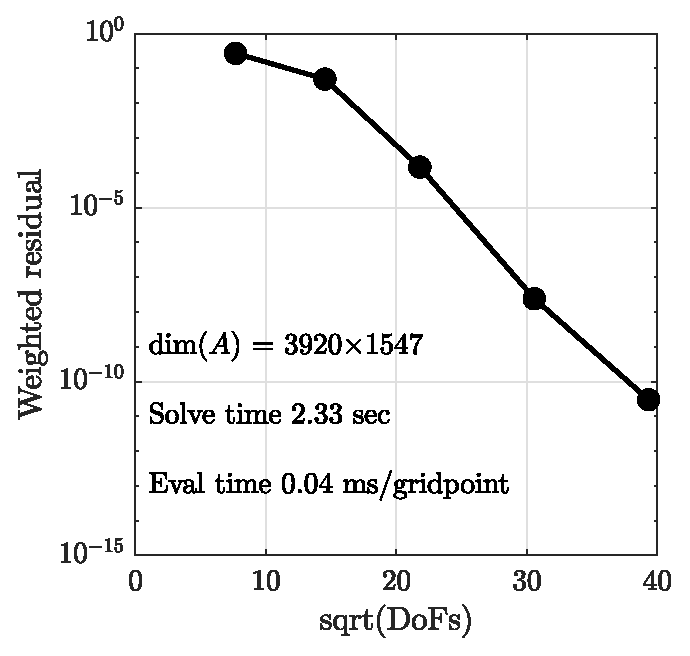
\includegraphics[width=0.4\linewidth]{Figures/step_conv}

	\caption{Stokes flow over a step.}
	\label{fig:step}
\end{figure} 
\end{example}

\section{Unbounded domains \label{sec:unbounded}}


\begin{figure}[H]
	\centering
	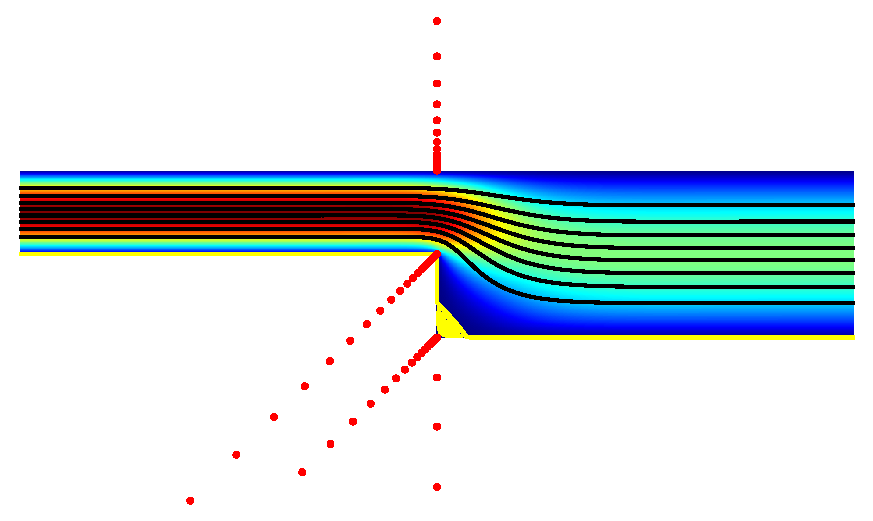
\includegraphics[width=\linewidth]{Figures/chan}
	
	\vspace{2em}
	\begin{minipage}{0.45\linewidth}
		\centering
		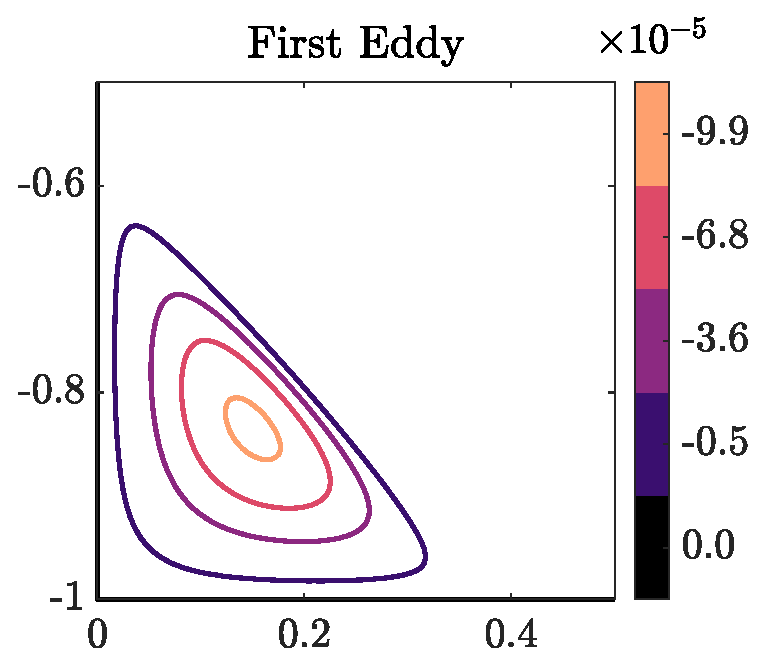
\includegraphics[width=\linewidth]{Figures/chan_eddy}
	\end{minipage}
	\hfill
	\begin{minipage}{0.45\linewidth}
		\centering
		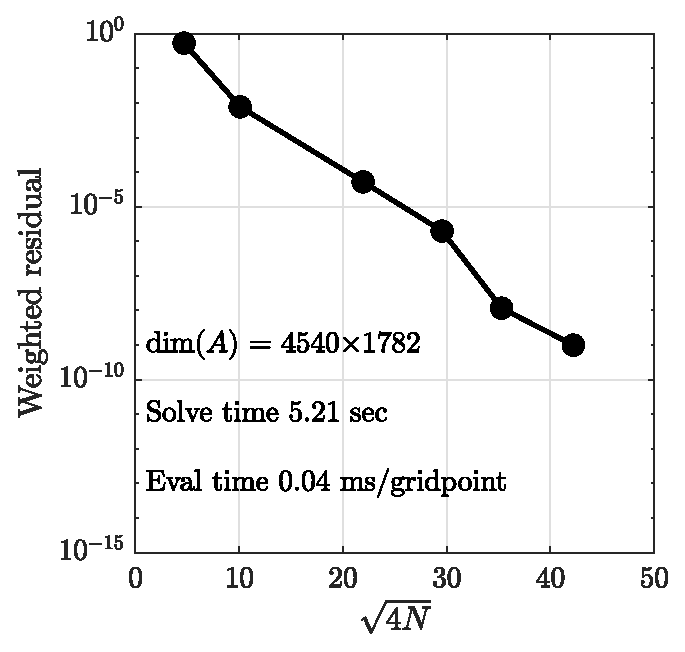
\includegraphics[width=\linewidth]{Figures/chan_conv}
	\end{minipage}
	

	\caption{Stokes flow inside an infinitely long pipe with an expansion.}
	\label{fig:chan}
\end{figure} 

\section{Multiply connected domains \label{sec:multiply}}


